% SC2000 — Chapter 5: Expectation & Variance
\chapter{Expectation, Variance \& Concentration}
\label{ch:expectation}

\begin{quote}
\emph{``Expectation is what happens on average; variance is how far average can mislead you.''} An algorithm's \emph{expected} runtime may be $O(n\log n)$ while its worst case is $O(n^2)$ (quicksort). Without variance and tail bounds, ``on average'' is a half-truth.
\end{quote}

\noindent\fbox{\parbox{\dimexpr\linewidth-2\fboxsep-2\fboxrule}{%
\textbf{From zero: weighted averages.} Expectation is the centre of mass of a distribution; variance is its moment of inertia. We derive linearity (which needs no independence) and build Markov, Chebyshev, and Chernoff bounds---the tools that turn averages into guarantees.}}
\vspace{0.4em}

\section*{Learning Outcomes}
After this chapter you will be able to:
\begin{enumerate}[label=(L\arabic*)]
    \item compute $\mathbb{E}[X]$ and $\mathrm{Var}(X)$ from PMF/PDF or via indicators;
    \item apply linearity of expectation (with dependence) and variance addition (with independence);
    \item use LOTUS, covariance, and correlation correctly;
    \item compute moment-generating functions and read off moments from them;
    \item apply Markov, Chebyshev, and Chernoff/Hoeffding tail bounds;
    \item analyse expected runtime of randomised algorithms (e.g., quicksort, hashing).
\end{enumerate}

% ============================================================
\section{Expectation: Centre of Mass}
\label{sec:expectation}

\begin{definition}[Expectation] For discrete $X$, $\displaystyle\mathbb{E}[X]=\sum_k k\,P(X=k)$. For continuous $X$ with PDF $f$, $\displaystyle\mathbb{E}[X]=\int x f(x)\,dx$, when absolutely convergent. More generally $\mathbb{E}[g(X)]=\sum g(k)p(k)$ or $\int g(x)f(x)\,dx$ (LOTUS: Law Of The Unconscious Statistician).
\end{definition}

\emph{Intuition:} place mass $p(k)$ at position $k$ on a rod; $\mathbb{E}[X]$ is the balance point.

\begin{theorem}[Linearity of expectation] For any $X,Y$ and constants $a,b$,
\[
\mathbb{E}[aX+bY]=a\mathbb{E}[X]+b\mathbb{E}[Y],
\]
with \emph{no independence assumption}. Hence $\mathbb{E}[\sum_{i=1}^n X_i]=\sum_i\mathbb{E}[X_i]$.
\end{theorem}

This is the most-used trick in randomised analysis: break a count into indicators.

\begin{example}[Indicators] Let $X_i=\mathbf{1}_{\{\text{trial }i\text{ succeeds}\}}\sim\mathrm{Bernoulli}(p)$. Then $S_n=\sum X_i\sim\mathrm{Bin}(n,p)$ and $\mathbb{E}[S_n]=\sum\mathbb{E}[X_i]=np$ without summing the Binomial PMF. Similarly, coupon collector, hashing collisions, and quicksort comparisons all yield to indicators.
\end{example}

\begin{figure}[h]
\centering
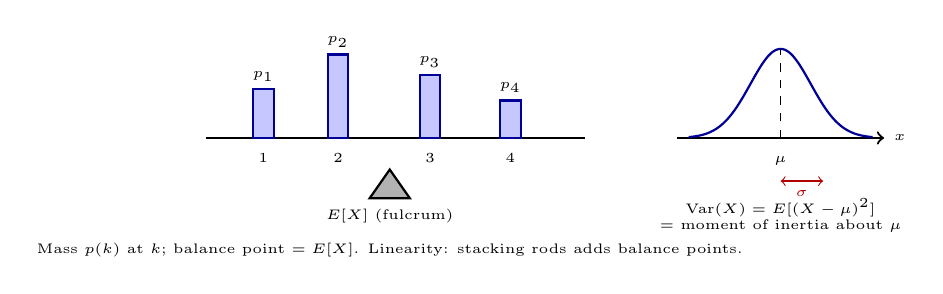
\begin{tikzpicture}[scale=0.73,every node/.style={font=\scriptsize}]
% Rod balance picture: expectation as fulcrum
\draw[thick] (-3.2,0)--(3.4,0);
\draw[thick,fill=gray!60] (0,-0.55) -- (-0.35,-1.05) -- (0.35,-1.05) -- cycle; % fulcrum
\node[font=\tiny] at (0,-1.35) {$\mathbb{E}[X]$ (fulcrum)};
% masses at positions
\foreach \x/\m/\lab in {-2.2/0.85/1, -0.9/1.45/2, 0.7/1.10/3, 2.1/0.65/4} {
  \draw[fill=blue!22,draw=blue!60!black,thick] (\x-0.18,0) rectangle (\x+0.18,\m);
  \node[font=\tiny] at (\x,-0.35) {$\lab$};
  \node[font=\tiny] at (\x,\m+0.22) {$p_{\lab}$};
}
\node[font=\tiny,align=center] at (0,-1.95) {Mass $p(k)$ at $k$; balance point $=\mathbb{E}[X]$. Linearity: stacking rods adds balance points.};
% Right: variance as spread
\begin{scope}[xshift=6.8cm]
\draw[->,thick] (-1.8,0)--(1.8,0) node[right,font=\tiny] {$x$};
\draw[thick,blue!60!black,smooth,domain=-1.6:1.6,samples=60] plot (\x,{1.55*exp(-\x*\x/0.55)});
\draw[dashed,thin] (0,0)--(0,1.55);
\node[font=\tiny] at (0,-0.40) {$\mu$};
\draw[<->,thin,red!70!black] (0,-0.75)--(0.74,-0.75) node[midway,below,font=\tiny] {$\sigma$};
\node[font=\tiny,align=center] at (0,-1.35) {$\mathrm{Var}(X)=\mathbb{E}[(X-\mu)^2]$\\= moment of inertia about $\mu$};
\end{scope}
\end{tikzpicture}
\caption{Left: expectation as centre of mass. Right: variance as spread (moment of inertia) about the mean.}
\label{fig:expectation-variance}
\end{figure}

Expectations of named distributions: $\mathrm{Bernoulli}(p):p$, $\mathrm{Bin}(n,p):np$, $\mathrm{Pois}(\lambda):\lambda$, $\mathcal{N}(\mu,\sigma^2):\mu$, $\mathrm{Uniform}[a,b]:(a+b)/2$, $\mathrm{Geom}(p):1/p$, $\mathrm{Exp}(\lambda):1/\lambda$.

\begin{remark}[Geometric vs.\ Exponential] Both are memoryless: $P(X>m+n\mid X>m)=P(X>n)$. Geometric counts discrete trials until success; Exponential measures continuous waiting time. They are the \emph{only} memoryless laws in their classes---a fact used to justify Exponential inter-arrival models in queueing.
\end{remark}

% ============================================================
\section{Variance, Covariance, Correlation}
\label{sec:variance}

\begin{definition}[Variance] $\mathrm{Var}(X)=\mathbb{E}[(X-\mathbb{E}[X])^2]=\mathbb{E}[X^2]-\mathbb{E}[X]^2\ge0$. Standard deviation $\sigma(X)=\sqrt{\mathrm{Var}(X)}$.
\end{definition}

\begin{theorem}[Properties] $\mathrm{Var}(aX+b)=a^2\mathrm{Var}(X)$. If $X,Y$ independent, $\mathrm{Var}(X+Y)=\mathrm{Var}(X)+\mathrm{Var}(Y)$. In general,
\[
\mathrm{Var}\!\left(\sum_i X_i\right)=\sum_i\mathrm{Var}(X_i)+2\sum_{i<j}\mathrm{Cov}(X_i,X_j),
\]
where $\mathrm{Cov}(X,Y)=\mathbb{E}[(X-\mu_X)(Y-\mu_Y)]=\mathbb{E}[XY]-\mathbb{E}[X]\mathbb{E}[Y]$. Correlation $\rho=\mathrm{Cov}(X,Y)/(\sigma_X\sigma_Y)\in[-1,1]$.
\end{theorem}

Independence $\Rightarrow$ $\mathrm{Cov}=0$ (uncorrelated), but converse fails. Variance adds only under uncorrelatedness.

\begin{example}[Binomial variance] $X=\sum_{i=1}^n X_i$ with $X_i$ i.i.d.\ $\mathrm{Bernoulli}(p)$, independent so $\mathrm{Var}(X)=n\,p(1-p)$.
\end{example}

\begin{theorem}[Jensen's inequality] If $g$ is convex, $g(\mathbb{E}[X])\le\mathbb{E}[g(X)]$; if concave, reverse. Example: $\mathbb{E}[X^2]\ge(\mathbb{E}[X])^2$ (since $x\mapsto x^2$ convex), which is exactly $\mathrm{Var}(X)\ge0$. For concave $\log$, $\mathbb{E}[\log X]\le\log\mathbb{E}[X]$---used in information theory (entropy bounds) and EM algorithms.
\end{theorem}

\begin{example}[Coupon collector expectation] Collect $n$ coupons, each trial uniform over $n$ types. Let $T_k$ be time to get $k$th new coupon after $k-1$ distinct seen; $T_k\sim\mathrm{Geom}(p_k)$ with $p_k=(n-k+1)/n$, $\mathbb{E}[T_k]=n/(n-k+1)$. Total $T=\sum_{k=1}^nT_k$, so $\mathbb{E}[T]=n\sum_{k=1}^n1/k=nH_n\sim n\ln n$. No joint distribution needed---linearity handles dependent stages via conditional expectations.
\end{example}

% ============================================================
\section{Moment-Generating Functions: A Distribution's Fingerprint}
\label{sec:mgf}
\emph{Intuition:} the MGF $M_X(t)=\mathbb{E}[e^{tX}]$ packs \emph{every} moment into one function: differentiating at $0$ unpacks them, $M_X^{(k)}(0)=\mathbb{E}[X^k]$. Two distributions sharing an MGF near $0$ are the \emph{same} distribution --- the MGF is a fingerprint (uniqueness theorem). Sums become easy: independent $X,Y$ give $M_{X+Y}=M_XM_Y$ (expectations multiply), so convolution turns into algebra.
\begin{example}[MGFs] $\mathrm{Bernoulli}(p)$: $M(t)=1-p+pe^t$, and $M'(0)=p=\mathbb{E}[X]$. $\mathcal{N}(\mu,\sigma^2)$: $M(t)=\exp(\mu t+\sigma^2t^2/2)$ --- reading the exponent recovers mean and variance. $n$ i.i.d.\ copies multiply MGFs, giving the $\mathrm{Bin}(n,p)$ MGF $(1-p+pe^t)^n$ in one line. The Chernoff bound below is Markov's inequality applied to $e^{tX}$ (whose mean \emph{is} the MGF), then optimised over $t$.
\end{example}

% ============================================================
\section{Tail Bounds: From Averages to Guarantees}
\label{sec:tail-bounds}

\begin{theorem}[Markov] If $X\ge0$, then for $a>0$, $P(X\ge a)\le\mathbb{E}[X]/a$.
\end{theorem}

\begin{theorem}[Chebyshev] For any $X$ with mean $\mu$, variance $\sigma^2$, and $k>0$,
\[
P(|X-\mu|\ge k\sigma)\le\frac1{k^2},\quad\text{or }P(|X-\mu|\ge t)\le\frac{\sigma^2}{t^2}.
\]
\end{theorem}

\begin{theorem}[Chernoff / Hoeffding, informal] For $S_n\sim\mathrm{Bin}(n,p)$ with $\mu=np$ and $0<\delta<1$,
\[
P(S_n\ge(1+\delta)\mu)\le\exp\!\left(-\frac{\delta^2\mu}{3}\right),\quad
P(|S_n-\mu|\ge t)\le2\exp\!\left(-\frac{2t^2}{n}\right)\ \text{(Hoeffding)}.
\]
Exponential tails vs.\ Chebyshev's $1/t^2$---vastly stronger for sums of bounded independent variables.
\end{theorem}

\begin{figure}[h]
\centering
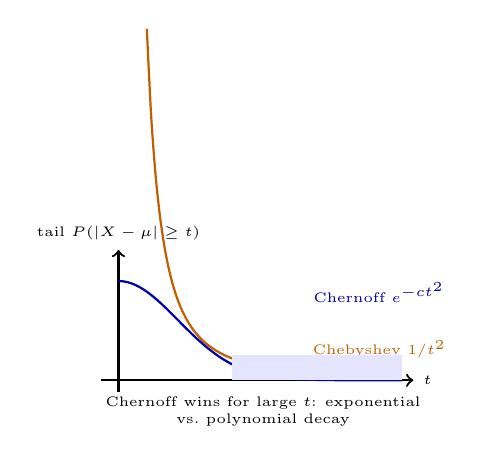
\begin{tikzpicture}[scale=0.72,every node/.style={font=\scriptsize}]
\draw[->,thick] (0,-0.2)--(0,2.3) node[above,font=\tiny] {tail $P(|X-\mu|\ge t)$};
\draw[->,thick] (-0.3,0)--(5.2,0) node[right,font=\tiny] {$t$};
% Chebyshev 1/t^2
\draw[thick,orange!75!black,smooth,domain=0.5:5,samples=60] plot (\x,{1.55/(\x*\x)});
\node[font=\tiny,orange!75!black] at (4.6,0.55) {Chebyshev $1/t^2$};
% Chernoff exp(-t^2)
\draw[thick,blue!65!black,smooth,domain=0:5,samples=60] plot (\x,{1.75*exp(-\x*\x/2.2)});
\node[font=\tiny,blue!65!black] at (4.6,1.55) {Chernoff $e^{-ct^2}$};
% shaded region
\fill[blue!10] (2.0,0) rectangle (5.0,0.45);
\node[font=\tiny,align=center] at (2.55,-0.55) {Chernoff wins for large $t$: exponential\\vs.\ polynomial decay};
\end{tikzpicture}
\caption{Chebyshev (polynomial) vs.\ Chernoff/Hoeffding (exponential) tail bounds. For sums of independent bounded variables, Chernoff dominates.}
\label{fig:tail-bounds}
\end{figure}

\begin{example}[Quicksort expected comparisons] Let $X_{ij}=\mathbf{1}_{\{\text{elements }i,j\text{ compared}\}}$. Then $P(X_{ij}=1)=2/(j-i+1)$ (they meet iff pivot is one of them first among $[i..j]$). Total comparisons $C=\sum_{i<j}X_{ij}$, so
\[
\mathbb{E}[C]=\sum_{i<j}\frac2{j-i+1}=2\sum_{k=1}^{n-1}\frac{n-k}{k+1}=2(n+1)H_n-4n\sim2n\ln n.
\]
No independence needed---linearity suffices.
\end{example}

% ============================================================
\section{Correlation, Covariance Matrices, and the Bias--Variance Lens}
\label{sec:cov-mat}
For a random vector $(X_1,\dots,X_d)$, the \emph{covariance matrix} $\Sigma_{ij}=\mathrm{Cov}(X_i,X_j)$ is symmetric positive semidefinite; diagonal entries are variances. Standardising gives the \emph{correlation matrix} $R_{ij}=\rho_{X_i,X_j}$. In computing, $\Sigma$ summarises feature redundancy: near-zero off-diagonals mean independent features, large $|\rho|$ suggests one can be dropped or merged. PCA finds the orthogonal rotation diagonalising $\Sigma$, ordering directions by variance.

\begin{example}[Hash probe length] With linear probing, probe count $P$ depends on load $\alpha$. $\mathbb{E}[P]\approx\frac12(1+1/(1-\alpha))$ for unsuccessful search; $\mathrm{Var}(P)$ grows sharply as $\alpha\to1$, so expectation alone understates tail latency---variance-aware sizing matters.
\end{example}

\begin{remark}[Why uncorrelated $\ne$ independent matters for ML] Many algorithms whiten data (decorrelate) and assume independence follows; Ch.~6 shows it does not. Always test joint factorisation, not just $\mathrm{Cov}=0$, before assuming Naive Bayes or mean-field approximations.
\end{remark}

% ============================================================
\section{Computing Expectation in Code}
\label{sec:code-expectation}

\begin{lstlisting}[language=Python]
import random, math

# Monte Carlo: estimate E[X] and Var(X) for Bin(100,0.3)
n, p, trials = 100, 0.3, 200000
samples = [sum(random.random()<p for _ in range(n)) for _ in range(trials)]
mean = sum(samples)/trials
var = sum((x-mean)**2 for x in samples)/trials
print(f"Empirical mean {mean:.2f} (true {n*p}), var {var:.2f} (true {n*p*(1-p):.2f})")

# Chebyshev vs Chernoff for Bin(100,0.5), t=15
mu, sigma2 = 50, 25
t = 15
print(f"Chebyshev bound P(|X-mu|>=15) <= {sigma2/t**2:.4f}")
print(f"Hoeffding bound <= {2*math.exp(-2*t**2/n):.4f}")  # 0.022
# Coupon collector: E[T] = n*H_n
import math as _m
for n in [10, 100, 1000]:
    Hn = sum(1/k for k in range(1, n+1))
    print(f"n={n} E[T]={n*Hn:.1f}")
\end{lstlisting}

% ============================================================
\section{Chapter Notes}
Linearity of expectation is de Moivre's insight; the indicator method is modern randomised-algorithms folklore (Motwani--Raghavan). Chebyshev (1867) and Chernoff (1952) bounds underpin PAC learning and randomised rounding. Quicksort analysis is Hoare (1962) refined by Sedgewick.

% ============================================================
\section{Exercises}
\label{sec:ch05-exercises}
\begin{enumerate}[label=E5.\arabic*, leftmargin=*, itemsep=0.8em]
\item \textbf{Indicators.} $n$ balls into $n$ bins uniformly. Let $X$ be the number of empty bins. Write $X=\sum X_i$ with indicators, compute $\mathbb{E}[X]$ and (harder) $\mathrm{Var}(X)$ via covariances. What happens as $n\to\infty$?
\item \textbf{LOTUS.} $X\sim\mathrm{Uniform}[0,1]$. Compute $\mathbb{E}[X^2]$, $\mathrm{Var}(X)$, and $\mathbb{E}[e^X]$ via LOTUS. Verify $\mathrm{Var}(X)=1/12$.
\item \textbf{Markov vs.\ Chebyshev vs.\ Chernoff.} For $S\sim\mathrm{Bin}(100,0.5)$, bound $P(S\ge70)$ with each inequality. Compute the exact tail via code and compare tightness. Which bound is closest?
\item \textbf{Correlation trap.} Give $X,Y$ dependent but $\mathrm{Cov}(X,Y)=0$ (hint: $X\sim\mathrm{Uniform}\{-1,0,1\}$, $Y=X^2$). Prove dependence yet zero correlation. What does this warn about ``uncorrelated = independent''?
\item \textbf{Quicksort variance (challenge).} Using the same $X_{ij}$ indicators, argue $\mathrm{Var}(C)=O(n^2)$ so Chebyshev gives concentration of $C$ around $2n\ln n$ within $O(n)$ with high probability.
\end{enumerate}
% End of Chapter 5
